%
% Modified by Sameer Vijay
% Last Change: Wed Jul 27 2005 13:00 CEST
%
%%%%%%%%%%%%%%%%%%%%%%%%%%%%%%%%%%%%%%%%%%%%%%%%%%%%%%%%%%%%%%%%%%%%%%%%
%
% Sample Notre Dame Thesis/Dissertation
% Using Donald Peterson's ndthesis classfile
%
% Written by Jeff Squyres and Don Peterson
%
% Provided by the Information Technology Committee of
%   the Graduate Student Union
%   http://www.gsu.nd.edu/
%
% Nothing in this document is serious except the format.  :-)
%
% If you have any suggestions, comments, questions, please send e-mail
% to: ndthesis@gsu.nd.edu
%
%%%%%%%%%%%%%%%%%%%%%%%%%%%%%%%%%%%%%%%%%%%%%%%%%%%%%%%%%%%%%%%%%%%%%%%%

%
% Chapter 4
%

\chapter{MUON VETO DEVELOPMENT}
\label{chap:muVeto}
\begin{comment}
Explain some cosmic ray basics - only the stuff relevant to our detector (1 muon per square foot per second and MIP -> landau energy distribution).
Discuss materials available for veto and basic design decision of WLS
\end{comment}

\section{Testing with \MgReaction}
\begin{comment}
Show results from first run and look at timing - hey it's all right!
Look at background - will need to improve
\end{comment}

\GeTargets cross-sections are predicted to be much lower than previous cross-sections measured with the neutron wall.  The differential cross-section of \MgReaction, however, is on the order of 1~mb/sr and and has been well measured by \cite{Bohne_Mg}, making \Mg{26} a good candidate for testing the neutron wall.  The TOF spectrum at the forwardmost angle, 6$^{\circ}$, is shown in {\fig}~\ref{fig:MgTOF}.  The neutron peak has a width of 1.2 ns and is clearly visible against the background. 
% figure: Bar A TOF spectrum
\begin{figure}[htp]
\centering
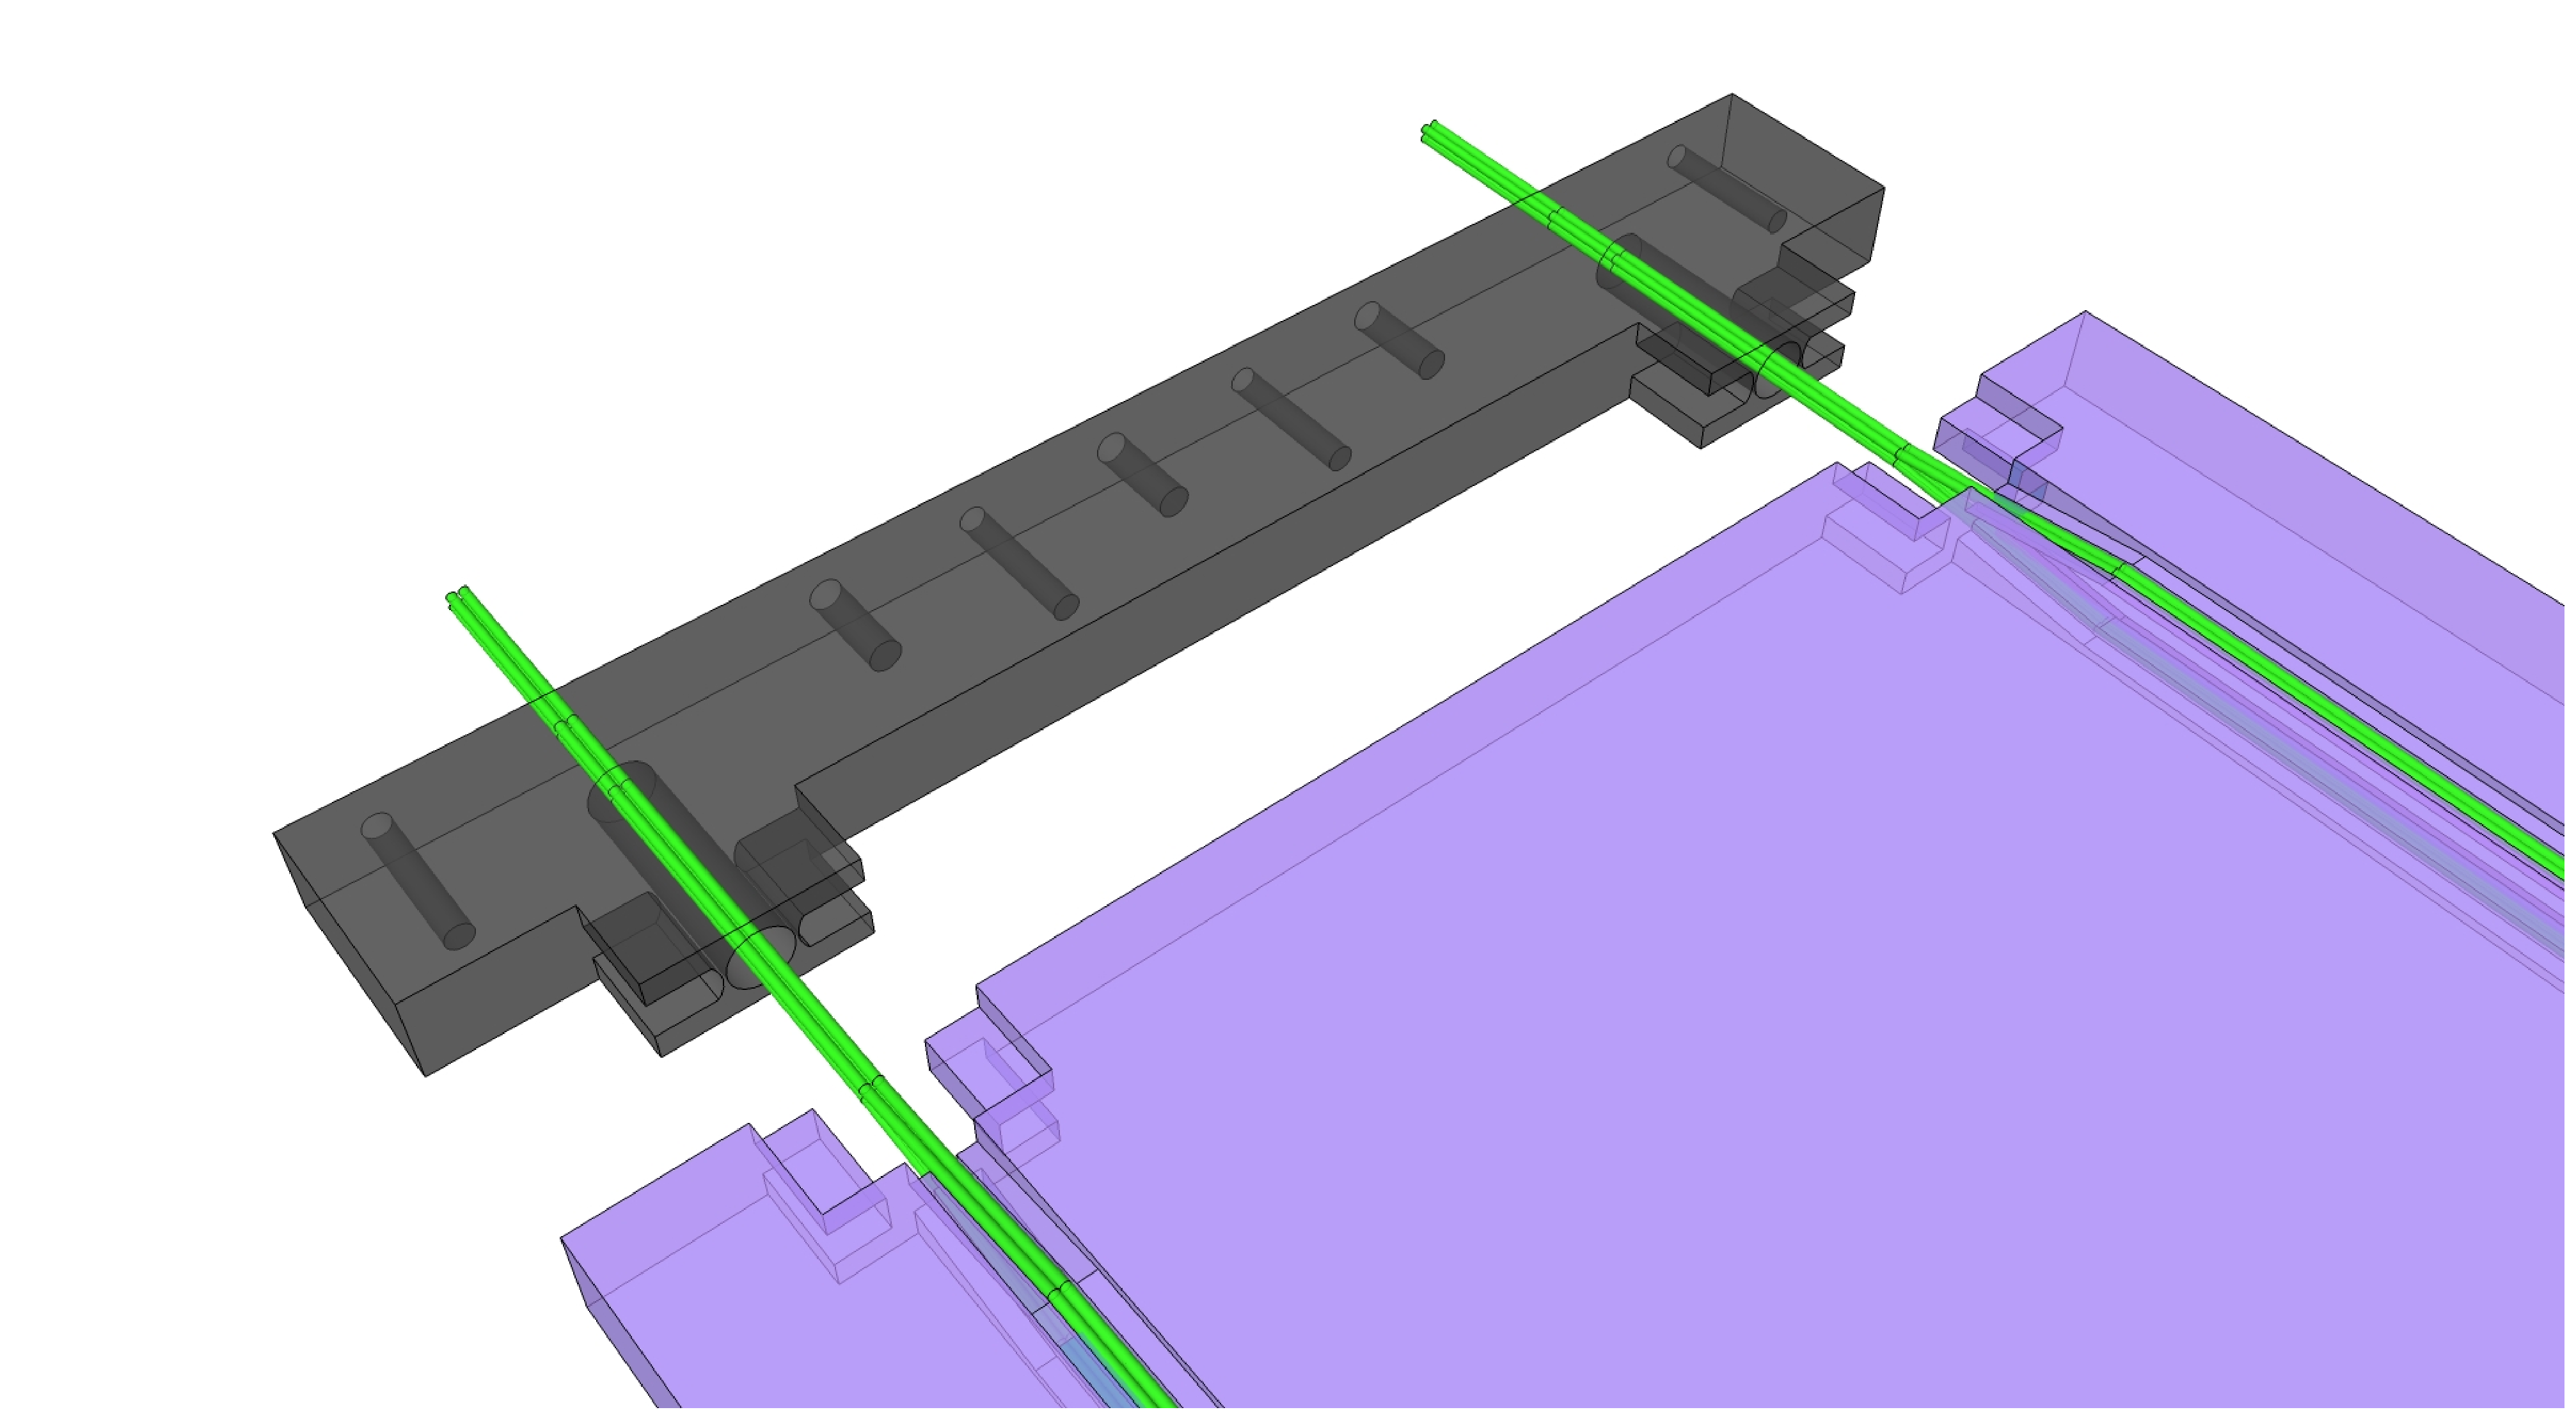
\includegraphics[width=1.0\textwidth]{figures/veto_assembly.eps}
\caption{The endcap will be glued to the scintillator after it is slid into place.}
\label{fig:paddleAssembly}
\end{figure}

The concerning thing about this data is that the neutron peaks at angles with low cross-sections do not stand significantly above the random background.  This has serious implications for the \GeTargets experiment, where DWBA calculations predict the cross-section to be $\sim$300~$\mu$b/sr.  Achieving 20\% uncertainty on the ground-state cross section requires either reducing the background or increasing the beam current.  Increasing the beam current was not feasible because of ion source limitations.  The background comes primarily from low-energy $\gamma$ radiation from the cement in the room and from muons produced by cosmic rays.  Neither vetoing nor shielding against $\gamma$-radiation would be effective since materials with high $\gamma$ interaction rates would also scatter incoming neutrons.  The muons, however, are charged and can be readily identified by their high interaction rate with nearly any material.  We therefore seek to reduce the muon component of the random background.

A practical solution to the muon background is to make a veto shield that registers the likely presence of a muon.  The events identified as muon events can then be discarded.  Distinguishing between muons and non-charged particle interactions using additional scintillator material is possible because of the difference in likelihood of interaction.  
\begin{figure}[hp]
\centering
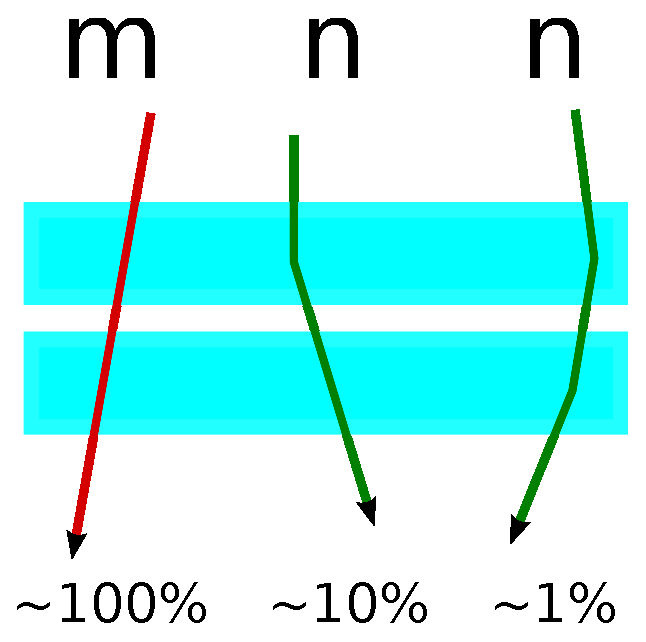
\includegraphics[width=0.4\textwidth]{figures/simpleVeto.eps}
\caption{The charged muon has a nearly 100\% chance of leaving a detectable signal in both scintillators, while the neutron, lacking charge, is much less likely to interact in even one of the scintillators.  The likelihood of detecting a neutron interaction depends on both the thickness of the scintillator and the threshold of the detector; for a 5 cm thick scintillator with a threshold at approximately the Th edge, the likelihood of detecting a 20 MeV neutron is about 10\%.}
\label{fig:simpleVeto}
\end{figure}
The energy distribution of muons incident on the neutron detector peaks at 100 GeV/C \cite{PDG}, so that most of the muons traveling through the detector are Minimum Ionizing Particles (MIP's).  This means that their energy loss is proportional to their path length in that material.  Muons at these energies deposit 1 MeV/cm2/g \cite{PDG}.  The detector consists of plastic with a density of ??, so the muons can deposit between 0.5 MeV to 80 MeV depending on their path through the plastic.  While the charged muon will trigger both detectors provided its path deposits energy above the detector threshold, the neutron is highly unlikely even to interact in both detectors.  The bars of the neutron detector are 5 cm thick; the chance of detecting a 20 MeV neutron when the detection threshold is at approximately the Th edge is 10\%, making the chance of a neutron interacting in two bars only 1\%.  If the muon veto is made of a thinner bar of scintillator, the probability of a detectable neutron interaction in both drops further.  By placing a thin ($\sim$1 cm) scintillator over the neutron detector bar, it is possible to identify muons to an accuracy of at least 99\%.  Note that such a veto does not identify $\gamma$ radiation because it has an efficiency similar to neutrons in BC408.

\section{Light Collection with WLS}
\begin{comment}
Describe light collection with WLS
Explain why we loop the WLS and collect light from both ends
Discuss the light limitations of light guides (Liouville) and ways to increase light collection with WLS (more!)
Describe fragility of WLS, how some efforts make custom plastic clamps to make it robust, how this doesn't work for you so you made a break and attached a cable.  Discuss signal loss.
\end{comment}
The scintillator bars of the neutron detector are outfitted with two PMT's, each coupled to its end via a non-scintillating light guide.  Having two PMT's is essential both for good timing information and also to lessen the position sensitivity of the signal.  Instrumenting the veto scintillators in this way was not feasible.  Fitting a top and bottom PMT to each veto bar would require 32 PMT's and lightguides, along with independent power supplies for each.  Instead, wavelength-shifting fiber (WLS) was chosen to collect the light.

WLS collects light by absorbing broad-spectrum radiation and re-emitting that light in the green.  It is possible to coat the fiber with material with an index of refraction that guarantees total internal reflection for green light, and so the light bounces in the fiber until it reaches a detector.  WLS largely eliminates position sensitivity because it can be arranged on the detector so that no part is distant from the collecting fiber [cite??].  Because the fiber is fairly flexible, its pattern on the detector can be designed so that the fiber exits the plastic in a single bundle, allowing instrumentation with only one PMT.

Possible disadvantages to WLS are signal intensity [cite??] and fragility of the fiber.  Sufficient light intensity to boost the signal above the noise is a serious concern, and can be overcome by using many WLS strands to collect light [cite NASA thing, show picture?].  The fragility of the WLS is more difficult to remedy.  To maximize light collection, the fiber on the detector should bee taken directly to the PMT, which should be as close to the plastic as possible to minimize signal attenuation.  In some designs [CITE!], this is acheived by enclosing the fiber run to the PMT in a stiff cast.  The design for the neutron wall needed flexibility in PMT placement, making a fixed support between the detector and PMT impractical.  Several attempts were made to run the WLS collection fiber directly from the scintillator to the PMT, but even with careful handling, the fiber quickly degraded and eventually snapped.  Such degredation would have left no way to access the veto's signals and was unacceptable.  The decision was made to sever the WLS at the end of the plastic and make a robust cable to attach to the WLS and carry the signal to the PMT.  While severing the WLS causes significant light loss, it ensures durability.  The details of this design are discussed in the next section.  

\section{Paddle Design}
\begin{comment}
Schematics
Tolerances
Making sure the transmit cable lines up with the paddle WLS fibers!  Dowels.  Tolerance doesn't actually need to be that good
connecting cable with PMT
cable design - hosing for protection
\end{comment}

The main components of a veto paddle are the scintillator and WLS, which does the actual detection, the endpiece that glues onto the scintillator, which fixes the position of the WLS coming off the scintillator, and the cable, which connects to the WLS and carries the signal to the PMT.  Each piece is discussed in this section.

The scintillator material itself is $\sim3/8$'', thinner than the bars of the neutron detector.  This is desirable because we don't want the neutrons to interact with material other than the neutron detector, but the thin material can still be efficient at detecting muons.  The fiber is glued to the paddle in a ``U'' shape as in {\fig}~\ref{fig:paddle}.  This is done to maximize light collection.  Light absorbed by the fiber propagates in both directions along the fiber axis; if one end of the fiber terminates, the light must reflect off the surface and travel back to the PMT, and light loss occurs both at the reflection and there's attenuation along the path.  Light loss at the terminating surface can be lessened somewhat with the application of reflective paint [CITE] and more so by silvering the surface [CITE], but a simpler method of recovering the light is to loop the fiber on the scintillator so that both ends can terminate at the PMT, allowing collection of light regardless of its travel direction.  With such a design, care must be taken to avoid extreme bending of the WLS, as it is easily damaged.  The bend radius chosen was ?? cm, which seemed to have no adverse effect on the WLS.

In general, the design goal was to maximize light collection while ensuring durability.  We could see that occasionally there was a default in the WLS cladding and were concerned that some fiber would suffer from more light loss than others.  The solution, using multiple strands of fiber to collect light, was intended to buffer the detector from chance defects in the WLS.  Using multiple strands of fiber also increases light collection, as found in [CITE!].  In general, light collection increases as more WLS is added to the surface, and there is not noticable position sensitivity if no part of the scintillator material is more than $\sim$5~cm from WLS fiber.  While more fiber could have been added to the surface of the scintillator, it already covered the surface and provided sufficient signal, shown in {\fig}~\ref{fig:vetoSignal}.  Furthermore, the WLS was glued into a channel machined into the scintillator to keep it from being damaged.  While more WLS fiber could increase the light collection, increasing the fiber on the surface would have meant machining away more scintillating material.  We did not want to reduce the possible energy deposition of the muons, as this was already quite low due to the thinness of the scintillator.

An endcap fitted to the scintillator helps protect the WLS and also ensures the WLS location, allowing good alignment to the fibers in the cable.  The endcap minimizes possible WLS flexing by connecting to machined indents in the scintillator with a press fit.  Because the endcap extends into the scintillator, bending the fiber perpendicular to its axis is essentially eliminated.  Scintillator is also machined away from the fiber's entrance to the endcap to avoid point pressure.  Once the endcap is slid onto the scintillator, it is glued in place, not to secure it to the scintillator, but to fix the WLS in their holes completely so that the surface of the endcap can be polished without damaging the WLS.

The cable that transmits the light from the WLS to the PMT has three seperate parts.  A connector mates with the endcap attached to the scintillator and connects to the tubing, which is 2~m long and connects to a connector that attaches to the PMT.  At each interface between tubing and connector, the primary concern is that the stresses on the transmission fiber be small enough to not damage the fiber.  A hose barb attached to each connector allows the transmission fiber through and also allows the tubing to firmly connect without putting strin on the fiber.  Slightly stiff tubing (durometer rating = ??) was chosen to help limit the bend radius of the cable, further protecting the transmission fiber.  

The primary concern for the portion of the cable that attaches to the endcap is that each transmission fiber completely overlap its WLS fiber.  The diameter of the transmission fiber is ??~mm, larger than the ??~mm-diameter WLS fiber, which allows misalignment of ??~mm without greatly impacting light collection.  Tight-fitting dowels help align the region of the cables containing the fiber cluster.  This is particularly important because the connectors are machined from plastic and are not perfectly square - some connectors bow as much as 20 mils from normal.  The only regions that must be carefully aligned, however, are the fiber clusters, and the dowels constrain these regions to less than ?? mils, ensuring an alignment of ?? mm.

\begin{figure}[htp]
\centering
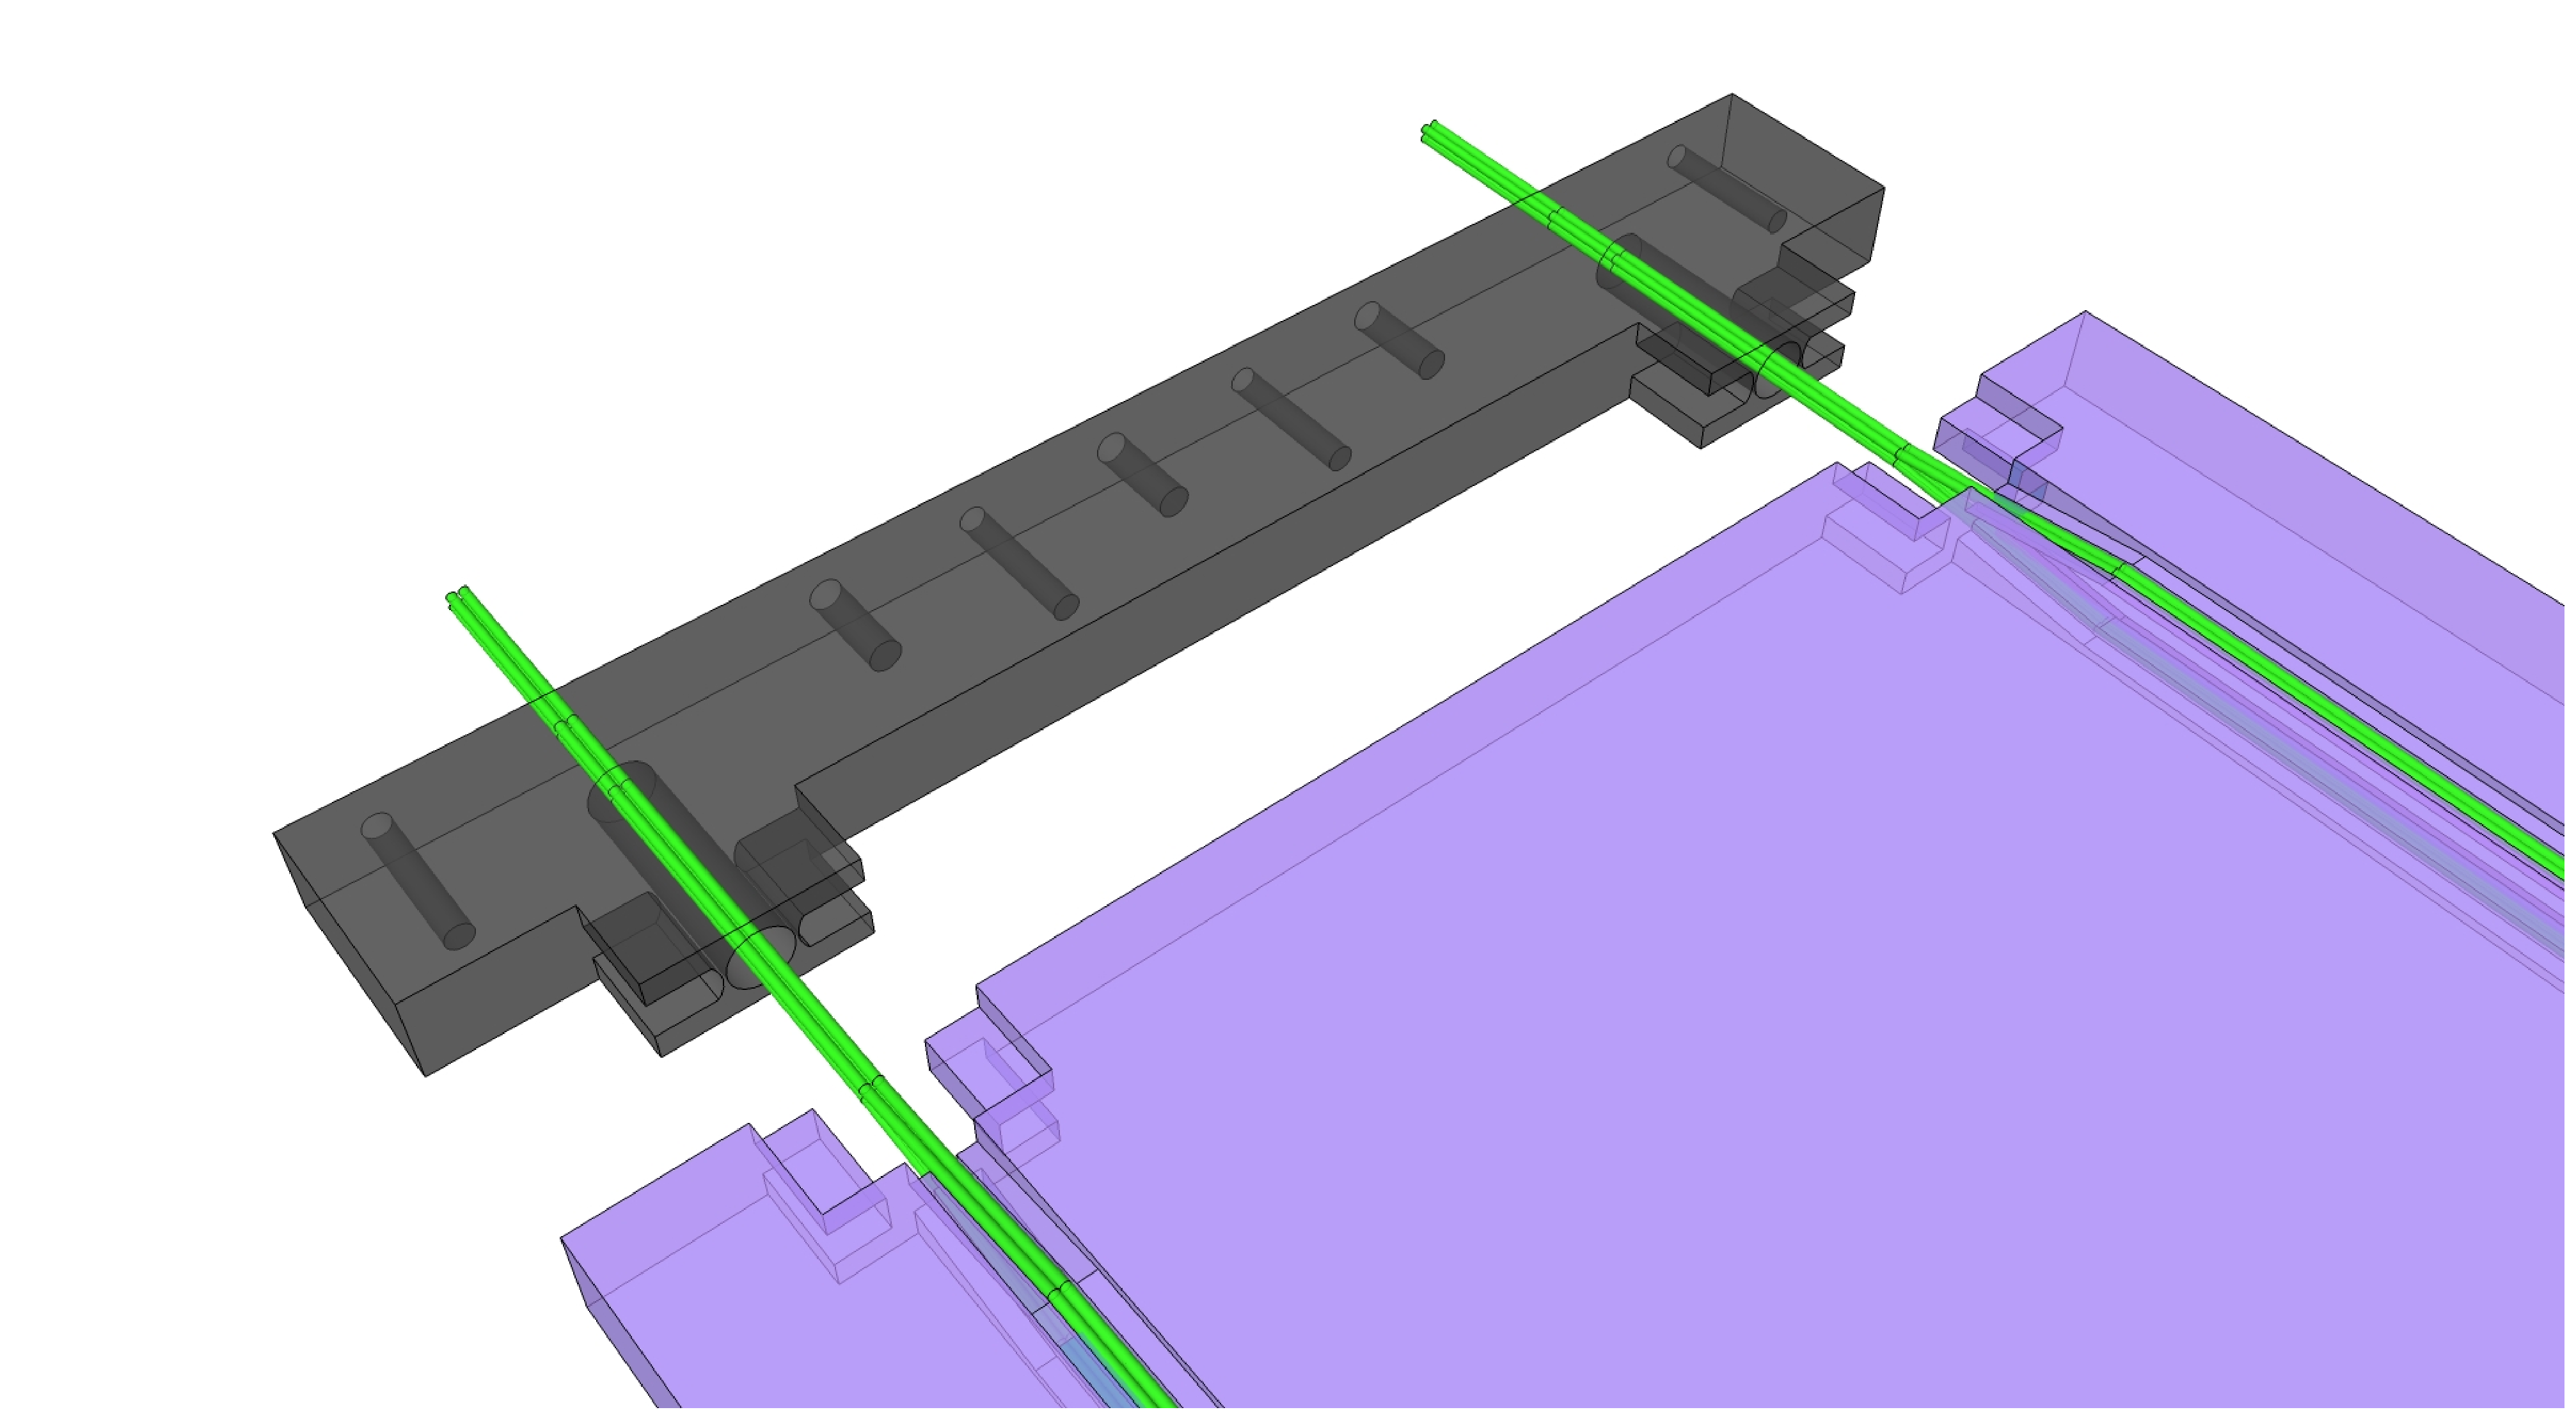
\includegraphics[width=1.0\textwidth]{figures/veto_assembly.eps}
\caption{The endcap will be glued to the scintillator after it is slid into place.}
\label{fig:paddleAssembly}
\end{figure}


\section{Paddle Performance}
\label{sec:singleVeto}

\subsection{tests on intrinsic efficiency}
\begin{comment}
Show signal from detector
Talk about first tests?  Can talk about sensitivity to geometric alignment of trigger paddles ...
Maybe mention this and then be like, ``this is why we decided to look at the efficiency this other way that was less sensitive''
except you weren't able to do further tests so you'll just have to say the limits you got
\end{comment}
The intrinsic efficiency of the paddles can be tested by requiring a coincidence with several paddles.  The several-detector coincidence identifies signals as muons.  If the coincidence paddles are arranged so that the path of any muon intersecting all the veto paddles must also intersect the volume of the veto paddle, the efficiency measured is the veto's intrinsic efficiency, separated from its geometric coverage of whatever detector it is vetoing.

In practice, arranging the available scintillator to force muons through the test volume was difficult because the available scintillator was instrumented with bulky lightguides and could not be laid directly on the test volume.  A simple cosmic ray simulation program helped determine an arrangement that maximized geometrical efficiency.  This arrangement, however, was extremely sensitive to placement; measured efficiency of the same bar could change from 98\% to 75\% with a displacement of a few centimeters.
\begin{figure}[htp]
\centering
\includegraphics[width=1.0\textwidth]{figures/efficiency_test.eps}
\caption{This arrangement of coincidence material ensures that muons triggering all coincidence detectors must also travel through the veto paddle.}
\label{fig:efficiencyTest}
\end{figure}

The efficiency was measured by counting how often the veto paddle had a detectable signal when all the coincidence material registered a coincidence.  Assuming the muon was constrained to travel through the veto paddle volume, the ratio gives the efficiency.  The DAQ Event signal was a logic pulse resulting from the coincidence of the coincidence paddles.  This logic pulse also acted as a Start for a TAC.  The TAC stop signal was a delayed, discriminated veto paddle signal.  The outgoing TAC signal was sent to an analog to digital converter (ADC) for integration.  Signals from the veto paddle coincident with the other scintillators show up in the timing spectrum as a peak at the time of the delay.  The integral of this timing peak divided by the number of event triggers gives the efficiency.
% figure: the considerably complicated spectrum
\begin{figure}[htp]
\centering
\subfloat[][]{
   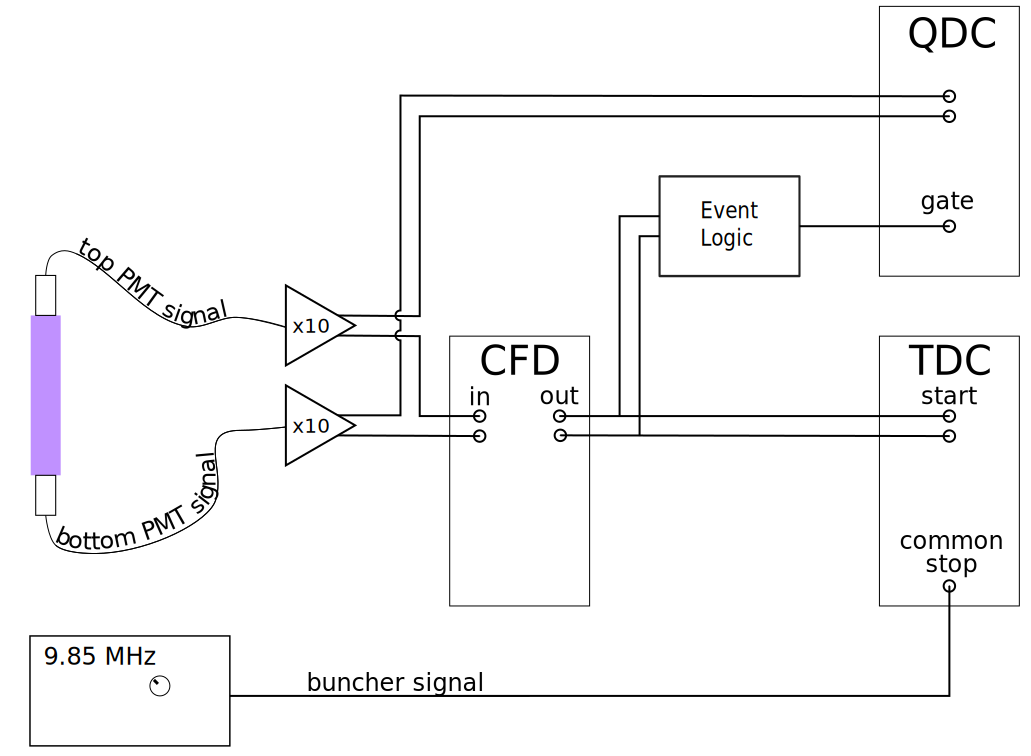
\includegraphics[width=0.45\textwidth]{figures/vetoTest_electronics.eps}	
}
\subfloat[][]{
	\includegraphics[width=0.45\textwidth]{figures/vetoTest_timing.eps}
}
\caption{The location of the timing peak is set by the delay introduced to the discriminated veto paddle signal.  Integrating the timing peak gives the number of muons that generated an observable signal in the veto paddle.}
\label{fig:vetoTestElectronics}
\end{figure}

Testing the efficiency of the veto paddle with this setup was not ideal because the geometrical efficiency was very sensitive to the placement of the coincidence detectors; measured efficiency of the same bar could change from 98\% to 75\% when one of the coincidence detectors was shifted by as little as a few centimeters.  However, this setup was useful in testing the effect of the cable polishing, cable out-of-true-ness, and the condition of the plastic scintillator.  In general, all efficiency measurements fell between 94\% and 98\%: even the veto paddles made of the most badly damaged plastic were as efficient as the veto paddles made from the plastic in excellent condition.  No statistically significant differences were seen between cables with the most and the least amount of bowing.  Polishing the cables with the bull-nose single-crystal diamond increases detection efficiency by $\sim2$\%, although it should be noted that the change may have been due to correlated noise in the system rather than to improved light transmission.  The discriminator threshold, set to its lowest value, gave an efficiency of 98\% compared to 94\% when set to its highest value.

Testing the position dependence of the efficiency using the setup described above was not practical due to its sensitivity on positioning.  Instead, the response of the veto paddles to a loosely collimated $\gamma$ source was tested.  Counting detected $\gamma$ radiation showed a deviation of less than 8.5\% over the veto paddle.  While this is not a measurement of the position dependence of the muon efficiency, it does limit the efficiency change over the paddle since muons typically deposit at least double the energy of the $\gamma$ radiation from the $^{60}$Co source.  See {\fig}~\ref{fig:positionDependence} for the variation of the efficiencies.
\begin{figure}[htp]
\centering
\includegraphics[width=1.0\textwidth]{figures/vetoTest_positionDependence.eps}
\caption{The dependence of the number of detected events on the position of a loosely-collimated $^{60}$Co source.  The spread is approximately 8.5\%.}
\label{fig:positionDependence}
\end{figure}


\subsection{On-Detector Efficiency}
\begin{comment}
Initial efficiency - would be nice to show this data
Describe different cosmics that hit the neutron bar but miss the veto - argh!
Discuss changes made to mounting to improve coverage - show new data (cosmics)
\end{comment}
Sixteen veto paddles were initially mounted on top of the neutron detector support structure to avoid removing (and potentially damaging) the heavy neutron detectors.  Each veto paddle was $\sim$2~cm offset from a bar in the neutron detector.  Running a test with 26Mg(3He,n) showed good cosmic rejection in the two innermost bars of each four-bar unit and worse rejection in the outer two bars by about 20\%, corresponding to double the cosmic background.  The outer bars act as additional veto for the inner bars, while the outer bars enjoy no such additional vetoing.  
\begin{figure}[htp]
\centering
\includegraphics[width=1.0\textwidth]{figures/initialBackground.eps}
\caption{Room background after rejection with the initial placement of the veto paddles.  Note that the high-background bars are those on the ends of each group of four.}
\label{fig:initialBackground}
\end{figure}

A simulation of the cosmic background indicated that the geometrical efficiency was very sensitive to the distance between the veto paddle and neutron detector bar as well as the distance between the bars of the neutron detector.   The bars in the neutron detector were moved as close as the mounting screws would allow, within 1~cm.  Instead of attaching the veto paddles on top of the retaining bars on the neutron detector, they were taped to the bars and both bar and veto paddle were supported together by the same retaining bar.  The separation between the bars of the neutron detector and their veto paddle is $\sim$0.5~cm due to stiff foam placed between the two to protect the WLS channels in the veto paddles.  Material was also added to the sides of the outermost neutron detectors.  The final setup is shown in {\fig}~\ref{fig:vetoSetup}.  These changes improved both the average and uniformity of the background rejection, as can be seen in {\fig}~\ref{fig:finalBackground}.
\begin{figure}[htp]
\centering
\includegraphics[width=1.0\textwidth]{figures/vetoSetup.eps}
\caption{The final arrangement of the veto paddles on the neutron detector.  The distance between the veto paddles and the bars of the neutron detector have been minimized.  Note also the addition of veto material on the sides of the neutron detector sub-units.}
\label{fig:vetoSetup}
\end{figure}

\begin{figure}[htp]
\centering
\includegraphics[width=1.0\textwidth]{figures/finalBackground.eps}
\caption{Room background after rejection by the veto.  Note that the average and the spread are both reduced from that of the initial setup.}
\label{fig:finalBackground}
\end{figure}

\section{Electronics}
\begin{comment}
Originally wanted to use timing information but there weren't enough channels
Bit Register - give example
discuss random rate and estimate how often you'll fire during a real event and also how often one bar will fire with something real, vetoing a real event
LeCroy 4532 - MALU - majority logic unit ``The status of up to 32 inputs can be monitored and recorded by issuing a strobe.  Since the inputs are edge-triggered, the strobe may be a gate of arbitrary duration.  Then any inputs which are on during any portion of the gate are recorded and stored in a pattern register.'' (from the manual).
\end{comment}
As mentioned above in {\sect}~\ref{sec:singleVeto}, tests on single veto paddles were done using a timing spectrum.  Recording time information for the full veto was not practical, and two bit registers were used instead.  A bit register has several inputs, each corresponding to a bit in an integer, and a gate.  When the gate is high, the bit register records the bit pattern built by the voltages on its inputs; its output is the integer corresponding to this bit pattern.  This integer is a unique representation of which bars fired during the time specified by the gate.  If the gate used is the Event signal from the neutron detector, the bit register will record which veto paddles fired during an event of interest.  Two 16-channel LeCroy 4532 bit registers were able to instrument all the veto paddles.  The gate signal was a 200~ns-wide copy of the event trigger.

Recording the integer generated by the bit register instead of the time of the signal relative to the beam bunch is a loss of information.  The maximum time difference between an event in the neutron detector and an event in the veto that will still be recorded in the bit pattern is the width of the gate signal, 200 ns.  This compares unfavorably to the timing spectrum, where even with a leading edge discriminator, the timing peak has a width of less than 5 ns.  The concern is that this loss of precision in timing information will lead to unacceptable vetoing of real events.  

Several sources contribute to non-beam-related background radiation, resulting in a beam-off rate in a neutron detector bar of $\sim$1000~Hz.  While some of these events are due to muons, but they have a rate of 1~Hz/ft$^2$ and are therefore a small part of the beam-off noise rate.  The beam-off rate, then, serves as a suitable rate with which to calculate an upper bound for the rejection of beam-related events.  The probability that a noise event will occur within the window allowed by the bit register and veto a beam-related event is
\begin{equation}
\text{P(A)}\times\text{P(B)} = \text{R}_{\text{n}}\tau_{\text{bit reg.}\times\text{R}_{\text{beam}}\tau_{\text{beam}} = 1000\text{Hz}\times 200\text{ns}\times\text{R}_{\text{beam}}\times 1000\text{ns} = 2\times10^{-10}\text{R}_{\text{beam}},
\end{equation}
where A is a noise event recording in the bit register and B is a beam-related event that has triggered the DAQ.  The probability of a veto scales with the noise rate $\text{R}_{\text{n}}$ and beam-related event rate $\text{R}_{\text{beam}}$ as well as the time window of the bit register $\tau_{\text{bit reg.}}$ and DAQ event $\tau_{\text{beam}}$.  This fraction of vetoed events is less than 1\% and will not have any statistical significance, even with the timing resolution lost by moving to a bit register.  A schematic of the veto electronics is shown in {\fig}~\ref{fig:vetoElectronics}.  Note that no changes to the DAQ other than the addition of the bit register are required.
\begin{figure}[htp]
\centering
\includegraphics[width=1.0\textwidth]{figures/vetoElectronics.eps}
\caption{The integration of the veto electronics with the existing DAQ.  The bit register is used in the data analysis.  Scalers are also added for run-time monitoring.}
\label{fig:vetoElectronics}
\end{figure}
 

\section{Beam Tests}
\begin{comment}
What data should I show?  Old Mg vs. New Mg?  Or New Mg with no veto vs.  New Mg with veto?
show the vetoed spectrum - put a limit on how much real signal is rejected?
\end{comment}
The background rejection of the assembled veto system is approximately 90\% as can be seen in {\fig}~\ref{fig:veto_26Mg}.  The rejection is strongly dependent on energy cuts placed on data; with lower energy cuts, gamma radiation contributes significantly to the background, and the veto is not effective.  90\% rejection is typical of cuts that are above the thorium edge.  Although such a high bound on the energy discards many neutron events, it also rejects more of the background $\gamma$ radiation and maximizes the signal/background ratio.See figure ?? for a description of the rejection as a function of the energy cut. 

\begin{figure}[htp]
\centering
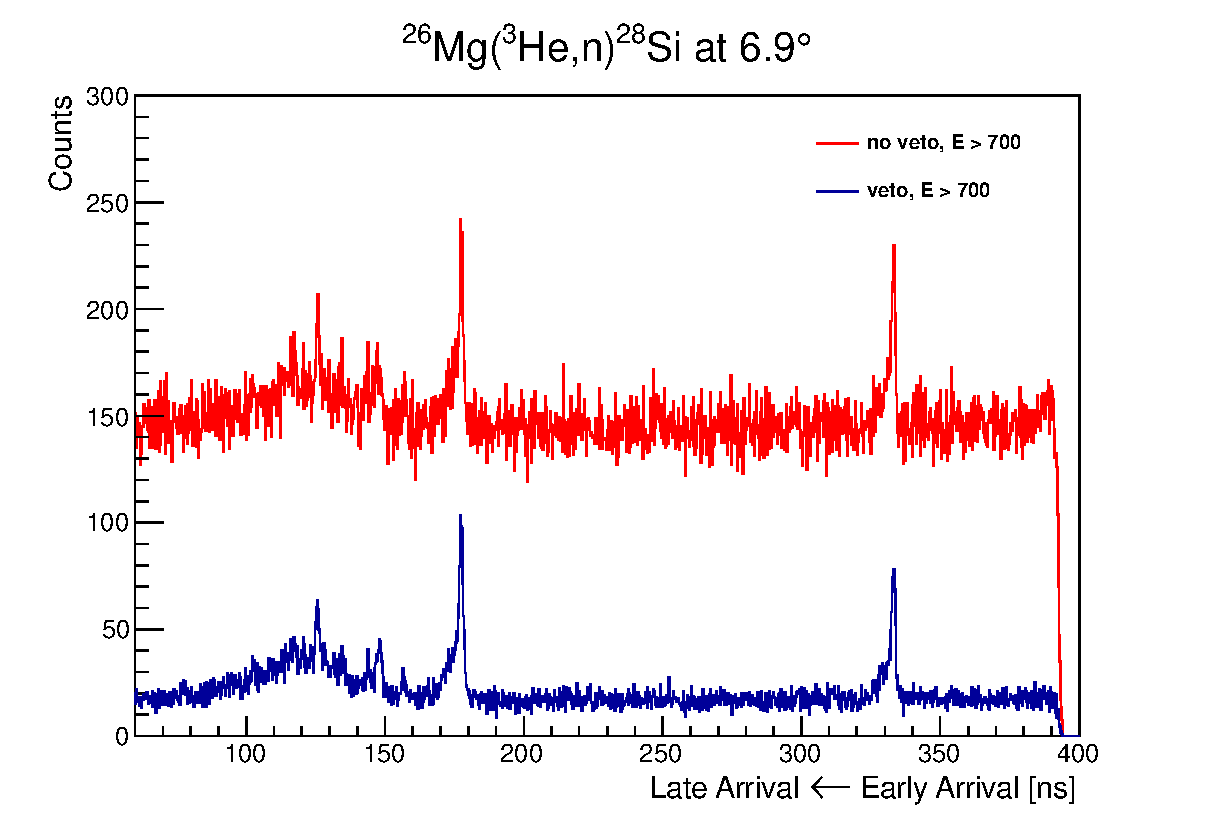
\includegraphics[width=5in]{figures/veto_26Mg.eps}
\caption{\label{fig:vetoData}The effect of the veto on the $^{26}$Mg($^3$He,n) data.}
\label{fig:veto_26Mg}
\end{figure}

The reduced background significantly improves the data we were able to obtain on \MgReaction.  Errors on the ground state transition were reduced from ?? to ??.  Most importantly, the signal strength that we now have 2$\sigma$ sensitivity to when running at a beam current of ?? for one week is ??, down from ??.  This is crucial for investigating the distribution of the \zp state in \GeTargets.

\subsection{Rejected Signal}
\begin{comment}
Two causes for rejected signal
1. the bars are ganged together; could get a signal in one veto bar that does not mean there was a cosmic in its adjacent neutron detector
2. randoms

can place a limit on randoms, reals, and therefore good rejected signal
\end{comment}
While the achieved background rejection is excellent, it is important to consider how often the veto rejects real neutron events.  Such a rejection could occur when a neutron interacts in both the veto and the neutron detector, when the neutron detector sees a real signal and the veto triggers from an uncorrelated event such as a background gamma, or when a neutron interacting in the detector kicks out a proton that triggers the veto.  This last case should occur very rarely; this is the primary reason we chose to mount the veto on the front of the detector.  It is also possible for the veto to absorb a neutron that could otherwise interact in the detector.  In all cases, the vetoing of real events will result in timing peaks that sit on top of the flat, random background of the rejected events.  {\fig}~\ref{fig:rejectionTOF} shows the rejected events for all current \Mg{26} data; no peak is visible.  Given the background, this places a limit on the total rejection of real neutron events at ?? at a 90\% confidence level.  
\begin{figure}[htp]
\centering
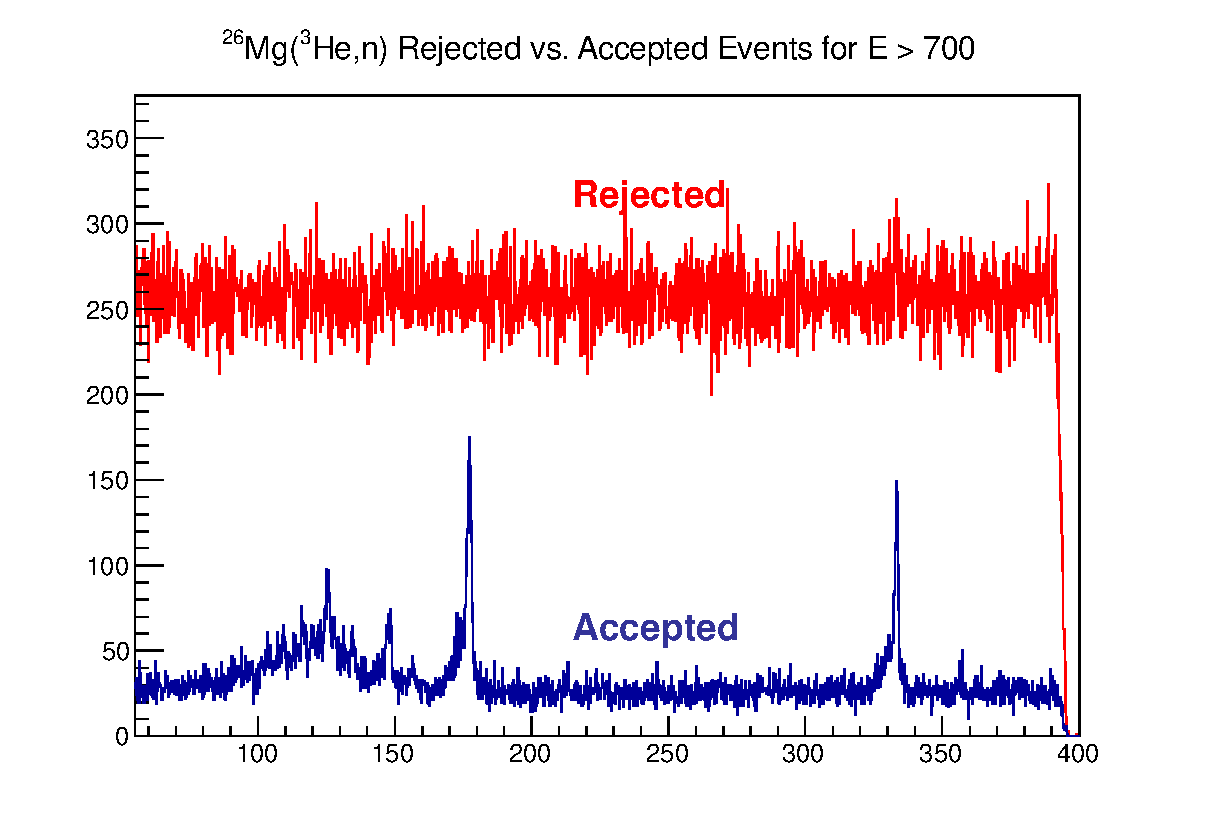
\includegraphics[width=5in]{figures/26Mg_rejection.eps}
\caption{\label{fig:rejection}A plot of the rejected events.  Peaks in the rejected spectrum are from real, vetoed events.  No neutron peak is visible; there is a small peak from rejected gamma events.}
\label{fig:rejectionTOF}
\end{figure}

Testing with \MgReaction demonstrates that the muon veto reduces background by $\sim$90\% and does not veto a significant number of beam-related events.  In addition to verifying the proper functioning of the veto system, this reaction also measures the efficiency of the neutron detector because the cross-section is well known.  These efficiency calculations, as well as the data from the \GeTargets experiments, will be discussed in the next chapter.


% % uncomment the following lines,
% if using chapter-wise bibliography
%
% \bibliographystyle{ndnatbib}
% \bibliography{example}
